\documentclass{../../text-style}

\texttitle{Базы данных}

\begin{document}

\maketitle
\thispagestyle{empty}

\section{Введение}

Без работы с базами данных не обходится ни одно веб-приложение и вообще ни одно приложение, которому надо что-то долго хранить и быстро получать доступ к данным. В принципе, люди долгое время прекрасно обходились обычными файлами, да и для задач типа хранения настроек приложения обычные файлы конфигурации вполне подходят. Но данные часто имеют сложную структуру, к ним приходится выполнять кучу разных видов запросов, к тому же данных, если они заводятся в вашем приложении, быстро становится очень много и они перестают помещаться в оперативке.

Кстати, есть базы данных, а есть системы управления базами данных. БД --- это, собственно, данные вместе с их структурой, СУБД --- это программа, которая предоставляет к этим данным доступ и позволяет их редактировать (или их структуру). СУБД бывают концептуально разные, каждый подход имеет свои достоинства и недостатки:

\begin{itemize}
    \item Реляционные --- до сих пор самый популярный вид СУБД, использующий реляционную алгебру (\url{https://en.wikipedia.org/wiki/Relational_algebra}) для представления данных и операций над ними. Данные в реляционной модели представляются в виде \textit{кортежей} значений разных типов, объединённых в \textit{отношения} --- самые настоящие алгебраические отношения и кортежи, в простонародье называемые таблицами и строками. На отношениях определены алгебраические операции, которые принимают отношения и возвращают отношения, определены совершенно формально и их свойства хорошо изучены. Эти алгебраические операции выражаются операторами языка SQL, который достаточно прост, чтобы им мог пользоваться любой школьник, несмотря на то, что внутри происходит кошмарная алгебраическая наука. Операции достаточно выразительны, чтобы с данными можно было делать практически всё, что угодно, и при этом достаточно декларативны, чтобы СУБД могла сама решать, как исполнять запрос, оптимизируя его зачастую в тысячи раз по сравнению с наивной реализацией.
    \item Объектно-ориентированные --- хранят по сути сериализованные объекты и позволяют исполнять запросы в духе ``найти объект по шаблону''. Значительно менее выразительный язык запросов компенсируется удобством использования из объектно-ориентированных программ --- результатом операции становится не какой-то невнятный набор кортежей, которые ещё надо как-то загрузить в объектно-ориентированную модель, а самый настоящий объект, будто мы его хранили в памяти. К тому же, такие базы, как правило, проще в конфигурировании и использовании, так что очень популярны сейчас для хранения небольших объёмов данных или данных, не предполагающих сложных запросов.
    \item Иерархические --- СУБД, хранящие данные в виде дерева. Самый типичный нынче пример таких штук --- базы, хранящие данные в XML-документах. Для запросов там используется язык XQuery, работающий с выражениями на языке XPath. Для иерархических по своей природе данных такие штуки незаменимы.
    \item Другие --- например, дедуктивные базы данных, которые вообще не хранят данные, они хранят некоторый набор фактов и правила, по которым могут быть выведены остальные факты (например, см. \url{https://en.wikipedia.org/wiki/Datalog}). 
\end{itemize}

Наиболее популярны сейчас всё-таки реляционные и объектно-ориентированные базы данных, поэтому часто приходится решать, какую же из этих моделей использовать. Так что рассмотрим соображения, могущие повлиять на решение:
\begin{itemize}
    \item Реляционные
    \begin{itemize}
        \item Минусы --- сложность интеграции с объектно-ориентированным кодом. Реляционная модель данных концептуально построена по принципу ``сущность-связь'', где сущность --- это штука, у которой есть имя и атрибуты, могущие иметь значения, а связь --- это ссылка из одной сущности на другую. Это очень похоже на объекты и отношения между ними, так что, казалось бы, никаких проблем быть не должно, но нет: сущности не могут наследоваться друг от друга, например. Чтобы хранить в реляционной базе объекты двух разных классов, наследующихся от общего предка, потребуется либо две таблицы с атрибутами, куда раскопипащены атрибуты предка, либо три таблицы --- для предка и двух потомков, и явные связи между потомками и предком. При загрузке и сохранении таких ``объектов'' фактически приходится реализовывать наследование вручную. Ещё реляционные базы не могут в отношение ``многие ко многим'', потому что связь там --- это просто ссылка на строку в другой таблице, она может быть только одной. Для решения этой проблемы заводят вспомогательные ``таблицы-развязки'', хранящие в себе только набор связей.
        \item Плюсы --- выразительный язык запросов, который даже со всякими там таблицами-развязками позволяет выбрать именно те данные, что нужны, и представить их в более-менее удобном виде. Кроме того, запросы выполняются, как правило, очень эффективно, грамотный проектировщик схемы БД может сделать так, чтобы выборка из сотен гигабайт данных занимала всего доли секунды. Впрочем, неудачная схема БД может испортить скорость работы всего приложения очень серьёзно.
    \end{itemize}
\end{itemize}

\section{Реляционная модель данных}

Рассмотрим подробнее реляционную модель (без алгебраических деталей). Данные там хранятся в виде отношений, которые удобнее всего себе представлять как таблицы, как на рисунке~\ref{image:table} из Википедии.

\begin{figure}
    \begin{center}
        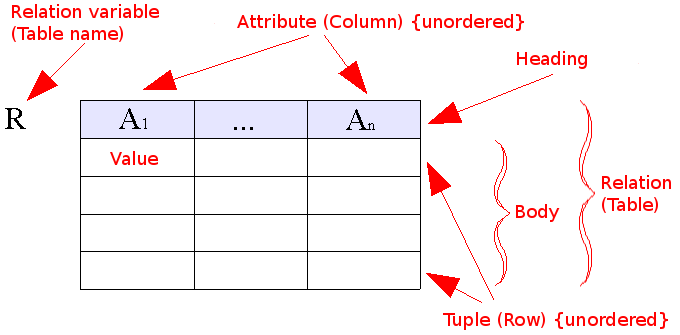
\includegraphics[width=0.7\textwidth]{relationalModel.png}
    \end{center}
    \caption{Отношение.}
    \label{image:table}
\end{figure}

У отношения есть имя (имя таблицы), у него есть колонки с именами и типами, и строчки, состоящие из, собственно, данных, лежащих в таблице. Пример таблицы с данными представлен в~\ref{table:tableWithData}.

\begin{figure}
    \begin{center}
        \begin{tabu} {| X[0.9 l p] | X[1 l p] | X[1 l p] | X[1 l p] |}
            \tabucline-
            CustomerID       & TaxID        & Name       & Address           \\
            \tabucline-
            \everyrow{\tabucline-}
            1234567890       & 555-5512222  & Munmun     & 323 Broadway      \\
            2223344556       & 555-5523232  & Wile E.    & 1200 Main Street  \\
            3334445563       & 555-5533323  & Ekta       & 871 1st Street    \\
            423242432        & 555-5325523  & E.F. Codd  & 123 It Way        \\
        \end{tabu}
    \end{center}
    \caption{Таблица с данными.}
    \label{table:tableWithData}
\end{figure}

\subsection{Ключи}

Если бы все данные, которые нужны программе, можно было хранить в одной таблице, то никакая реляционная алгебра была бы не нужна. Интереснее становится, когда данные имеют сложную структуру, требующую нескольких связанных таблиц. Например, список городов и список улиц, где каждая улица привязана к конкретному городу (рис.~\ref{table:citiesStreets}).

\begin{figure}
    \begin{center}
        CITY
        \begin{tabu} {| X[0.2 l p] | X[1 l p] |}
            \tabucline-
            ID      & Name \\
            \tabucline-
            \everyrow{\tabucline-}
            1       & Москва \\
            2       & Санкт-Петербург \\
            3       & Владивосток \\
        \end{tabu}
        \vspace{3mm}
        STREET
        \begin{tabu} {| X[0.2 l p] | X[1 l p] | X[0.7 l p] |}
            \tabucline-
            ID       & Name             & ID\_CITY \\
            \tabucline-
            \everyrow{\tabucline-}
            181      & Малая Бронная    & 1 \\
            182      & Тверской Бульвар & 1 \\
            183      & Невский проспект & 2 \\
            184      & Пушкинская       & 2 \\
            185      & Светланская      & 3 \\
            186      & Пушкинская       & 3 \\
        \end{tabu}
    \end{center}
    \caption{Таблицы с городами и улицами.}
    \label{table:citiesStreets}
\end{figure}

В принципе, всё можно было сложить и в одну таблицу (хранить в STREET просто названия городов), но, во-первых, это дупликация данных, во-вторых, города могут понадобиться кому-то ещё.

Как в базах данных работают ссылки на другие таблицы --- очень просто, на самом деле. Есть понятие ``ключ'', набор столбцов, уникально идентифицирующих любой кортеж в таблице. Первичный ключ --- это уникальный идентификатор в таблице с нашими данными, внешний ключ --- это уникальный идентификатор наших данных, сохранённый в какой-то другой таблице. В примере~\ref{table:citiesStreets} первичным ключом в таблице CITY был столбец ID, в таблице STREET тоже есть первичный ключ (и тоже ID), но есть и внешний ключ --- столбец ID\_CITY, где просто записаны первичные ключи городов, которым принадлежат улицы. 

Может показаться, что первичный ключ --- это всегда число, что-то вроде номера ячейки памяти, но нет, они бывают разные. Бывают естественные первичные ключи --- идентификаторы, присущие самим данным, например, номер паспорта или номер зачётки. Они уникальны по самой своей природе, поэтому вполне подходят в качестве первичных ключей. Бывают даже составные ключи --- ключи, состоящие из нескольких колонок. Например, название не идентифицирует город однозначно, но название страны, название региона плюс название города --- вполне себе уникальный идентификатор. Тогда в качестве внешнего ключа приходится использовать все значения, входящие в составной ключ.

Суррогатными ключами называются ключи, которых нет в предметной области, и их пришлось специально придумать, чтобы однозначно идентифицировать объекты (например, ID из~\ref{table:citiesStreets}). Они используюся чаще, чем естественные, потому что они заведомо уникальны --- например, MAC-адрес было бы разумно использовать как естественный ключ, но только до тех пор, пока нам не попадутся две сетевые карты с одинаковым MAC-адресом, который должен быть глобально уникальным. Кроме того, они компактнее, чем большинство естественных ключей. Но не очень хорошо работают в сценариях, когда требуется использовать данные из двух разных баз данных, так что естественные ключи всё-таки бывают полезны.

\subsection{Ограничения}

Базе данных можно сказать, что колонка --- это первичный ключ, тогда она будет сама проверять его уникальность (и даже генерить, если попросить). Это делается с помощью \textit{ограничений} --- свойств колонок в схеме БД. Первичные ключи описываются как ограничение PRIMARY KEY (чуть попозже будет понятно, куда это писать). Бывает ещё ограничение FOREIGN KEY, заставляющее СУБД проверять, что такой ключ действительно есть в таблице, на которую ссылается внешний ключ (сам ключ не ссылается, это просто значение, но в самом ограничении можно указать, о какой таблице идёт речь). Отметим, что кортеж, на который ссылается какой-то из внешних ключей, нельзя удалить (без \textit{каскадного удаления}, по крайней мере, когда удаляется и кортеж, и все кортежи, которые на него ссылаются, и все кортежи, которые ссылаются на них, и т.д.).

Есть ещё ограничение NOT NULL, заставляющее атрибут всегда иметь значение (по умолчанию значение любого типа может быть NULL, что означает отсутствие значения), и UNIQUE, что заставляет значение быть уникальным в своей колонке. Попытка вставить данные, которые нарушают уникальность, будет отклонена СУБД.

\section{SQL}

Теперь, собственно, про то, как работать с реляционными данными. Для этого чаще всего используется язык SQL (Structured Query Language). Он был специально спроектирован так, чтобы быть максимально простым и похожим на разговорный английский. 

\subsection{SELECT}

Самый известный, пожалуй, оператор SQL --- это SELECT (да, в SQL ключевые слова по традиции пишут капсом, хотя сам язык регистронезависимый, как Паскаль). SELECT позволяет выбрать данные по некоторому критерию из некоторой таблицы или некоторого набора таблиц, получив новую таблицу (это алгебраический оператор, мы хотим замкнутость, так что да, результат SELECT --- таблица). Несколько примеров из Википедии приведены на рис.~\ref{image:select}, подробное описание можно посмотреть на \url{https://www.w3schools.com/sql/sql_select.asp} (учтите, что почти каждая СУБД имеет свой диалект SQL, так что синтаксис и возможности могут немного различаться, но для часто используемых случаев всё будет работать везде).

\begin{figure}
    \begin{center}
        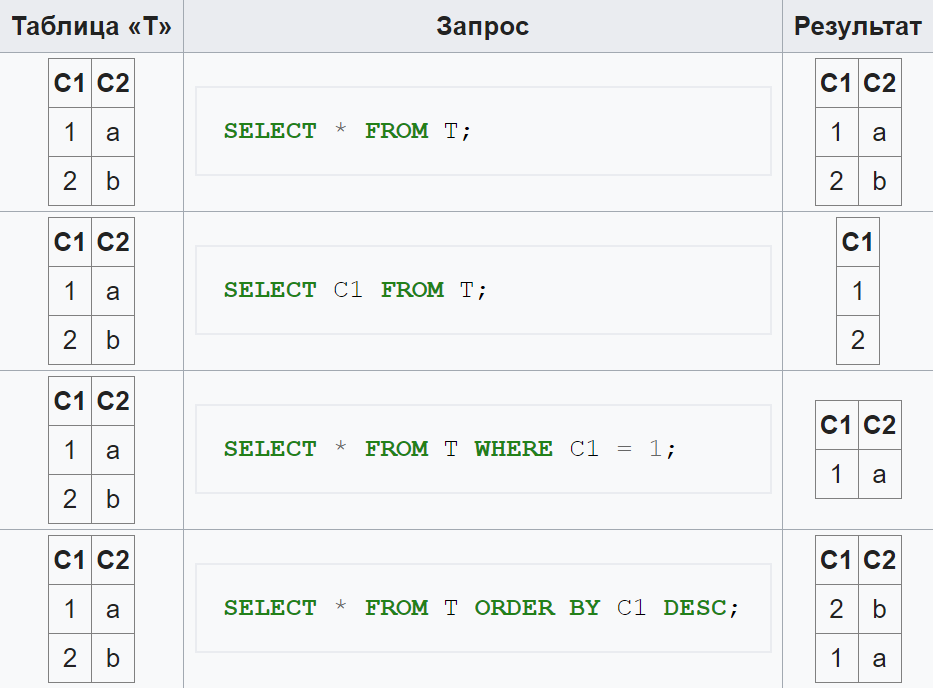
\includegraphics[width=0.6\textwidth]{select.png}
    \end{center}
    \caption{Оператор SELECT.}
    \label{image:select}
\end{figure}

Самое интересное тут, пожалуй, WHERE --- часть с предикатом, который определяет, какие кортежи попадут в результирующее отношение. Именно благодаря WHERE можно выбирать только те данные, которые нужны, и не грузить в оперативку все сотни гигов данных из базы.

SELECT поддерживает вложенные запросы и агрегатные функции. Например, 

\begin{minted}{sql}
SELECT isbn,
       title,
       price
FROM Book
WHERE price < (SELECT AVG(price) FROM Book)
ORDER BY title;
\end{minted}

Этот запрос выбирает книги с ценой, меньшей средней, и сортирует их по названию. AVG --- агрегатная функция, принимает имя колонки и возвращает среднее значение числовых данных в этой колонке. Обратите внимание на то, что все функции вызываются как запросы к БД, через SELECT.

\subsection{INNER JOIN}

Самая, пожалуй, важная функциональность SELECT-а связана с возможностью получать данные из нескольких таблиц сразу, объединяя результаты запроса в новую таблицу. Например, рассмотрим таблицы с рисунка~\ref{table:citiesPeople}.

\begin{figure}
    \begin{center}
        \begin{tabular}{c c}
            CITY & STREET \\
            \begin{tabu} to 0.3\textwidth {| X[0.2 l p] | X[1 l p] |}
                \tabucline-
                ID      & Name \\
                \tabucline-
                \everyrow{\tabucline-}
                1       & Москва \\
                2       & Санкт-Петербург \\
                3       & Владивосток \\
            \end{tabu}
            &
            \begin{tabu} to 0.5\textwidth {| X[0.5 l p] | X[1 l p] |}
                \tabucline-
                Name             & CITY\_ID \\
                \tabucline-
                \everyrow{\tabucline-}
                Андрей      & 1 \\
                Леонид      & 1 \\
                Сергей      & 2 \\
                Григорий    & 4 \\
            \end{tabu}
        \end{tabular}
    \end{center}
    \caption{Таблицы с городами и улицами.}
    \label{table:citiesPeople}
\end{figure}

Вот так можно получить названия городов, в которых живут люди:

\begin{minted}{sql}
SELECT * FROM Person INNER JOIN City ON Person.CityId = City.CityId
\end{minted}

То есть SELECT берёт данные из Person и City, дальше объединяет два кортежа, таких что их CityId совпадают, в один кортеж, и всё, что получилось, складывает в результирующую таблицу. Результат можно посмотреть в~\ref{table:citiesPeopleResult}.

\begin{figure}
    \begin{center}
        \begin{tabu}{| X[1 l p] | X[1 l p] | X[1 l p] | X[1 l p]  |}
            \tabucline-
            Person.Name  & Person.CityId  & City.Id  & City.Name       \\
            \tabucline-
            \everyrow{\tabucline-}
            Андрей       & 1              & 1        & Москва          \\
            Леонид       & 1              & 1        & Москва          \\
            Сергей       & 2              & 2        & Санкт-Петербург \\
        \end{tabu}
    \end{center}
    \caption{Результат запроса.}
    \label{table:citiesPeopleResult}
\end{figure}

Эта конструкция настолько часто используется, что работает и вот так:

\begin{minted}{sql}
SELECT * FROM Person, City WHERE Person.CityId = City.CityId
\end{minted}

\subsection{OUTER JOIN}

INNER JOIN не добавляет в результат данные, которым не нашлось ``пары'' в хотя бы одной из таблиц (это логично, с чего бы, для них ведь условие в WHERE не выполняется). Иногда всё же надо получить результат, включающий в себя все данные, включая те, для которых не нашлось соответствия. Это делает OUTER JOIN:

\begin{minted}{sql}
SELECT * FROM Person LEFT OUTER JOIN City ON Person.CityId = City.CityId
\end{minted}

Результат теперь получится таким:

\begin{center}
    \begin{tabu}{| X[1 l p] | X[1 l p] | X[1 l p] | X[1 l p] |}
        \tabucline-
        Person.Name  & Person.CityId  & City.Id  & City.Name       \\
        \tabucline-
        \everyrow{\tabucline-}
        Андрей       & 1              & 1        & Москва          \\
        Леонид       & 1              & 1        & Москва          \\
        Сергей       & 2              & 2        & Санкт-Петербург \\
        Григорий     & 4              & NULL     & NULL            \\
    \end{tabu}
\end{center}

Обратите внимание, что OUTER JOIN не симметричен --- сейчас в выдачу попал Григорий, но если бы мы записали таблицы в другом порядке, в выдачу бы попал Владивосток.

\subsection{CROSS JOIN}

Ещё бывает CROSS JOIN --- это на самом деле просто SELECT по нескольким таблицам без ON или WHERE. Что он делает, несложно догадаться --- просто объединяет всё со всем, строя фактически декартово произведение кортежей. Например, если написать

\begin{minted}{sql}
SELECT * FROM Person, City
\end{minted}

получится

\begin{center}
    \begin{tabu}{| X[1 l p] | X[1 l p] | X[1 l p] | X[1 l p] |}
        \tabucline-
        Person.Name  & Person.CityId  & City.Id  & City.Name       \\
        \tabucline-
        \everyrow{\tabucline-}
        Андрей       & 1              & 1        & Москва          \\
        Андрей       & 1              & 2        & Санкт-Петербург \\
        Андрей       & 1              & 3        & Владивосток     \\
        Леонид       & 1              & 1        & Москва          \\
        Леонид       & 1              & 2        & Санкт-Петербург \\
        Леонид       & 1              & 3        & Владивосток     \\
        Сергей       & 2              & 1        & Москва          \\
        Сергей       & 2              & 2        & Санкт-Петербург \\
        Сергей       & 2              & 3        & Владивосток     \\
        Григорий     & 4              & 1        & Москва          \\
        Григорий     & 4              & 2        & Санкт-Петербург \\
        Григорий     & 4              & 3        & Владивосток     \\
    \end{tabu}
\end{center}

Как правило, такой запрос  получается случайно, при этом СУБД честно пытается его выполнить, строит огромное декартово произведение и падает из-за недостатка оперативки.

\subsection{Таблицы-развязки}

Теперь, наконец, можно рассказать, как в реляционной модели реализуется отношение ``многие-ко-многим''. Например, мы хотим хранить данные о научных статьях и их авторах, но у статьи может быть много авторов и у автора может быть много статей. Тогда нам потребуется ещё одна таблица, которая будет хранить соответствие автора и статьи. Например,

\begin{center}
    \begin{tabular}{c c c}
        Author & AuthorArticle & Article \\
        \begin{tabu} to 0.25\textwidth {| X[0.2 l p] | X[1 l p] |}
            \tabucline-
            ID      & Name \\
            \tabucline-
            \everyrow{\tabucline-}
            1       & Терехов \\
            2       & Брыксин \\
            3       & Литвинов \\
        \end{tabu}
        &
        \begin{tabu} to 0.25\textwidth {| X[1 l p] | X[1 l p] |}
            \tabucline-
            AuthorId             & ArticleId \\
            \tabucline-
            \everyrow{\tabucline-}
            1   & 1 \\
            1   & 2 \\
            2   & 1 \\
            2   & 3 \\
            3   & 1 \\
            3   & 3 \\
        \end{tabu}
        &
        \begin{tabu} to 0.45\textwidth {| X[0.1 l p] | X[1 l p] |}
            \tabucline-
            ID      & Title \\
            \tabucline-
            \everyrow{\tabucline-}
            1       & Архитектура среды визуального моделирования QReal \\
            2       & Технология программирования \\
            3       & Среда визуального программирования роботов QReal:Robots \\
        \end{tabu}
    \end{tabular}
\end{center}

Наличие такой таблицы-развязки позволяет использовать её в WHERE (или ON) при выполнении SELECT-а. Например, как узнать все статьи Андрея Николаевича Терехова, зарегистрированные в нашей базе:

\begin{minted}{sql}
SELECT Article.Title FROM Author, AuthorArticle, Article 
    WHERE Author.Id = AuthorArticle.AuthorId 
        AND AuthorArticle.ArticleId = Article.Id 
        AND Author.Name = 'Терехов'
\end{minted}

Или как найти всех авторов статьи ``Среда визуального программирования роботов QReal:Robots'':

\begin{minted}{sql}
SELECT Author.Name FROM Author, AuthorArticle, Article 
    WHERE Author.Id = AuthorArticle.AuthorId 
        AND AuthorArticle.ArticleId = Article.Id 
        AND Article.Title = 'Среда визуального программирования роботов QReal:Robots'
\end{minted}

\subsection{INSERT, UPDATE, DELETE}

Вставлять новые данные в базу можно с помощью оператора INSERT. Выглядит это примерно так:

\begin{minted}{sql}
INSERT INTO City(Name) VALUES ('Казань');
\end{minted}

Указывается имя таблицы, в скобках имена столбцов, которые мы хотим задать, затем после VALUES значения, которые нужно сохранить в новый кортеж. Если не указали столбец, который может автогенерироваться (например, суррогатный первичный ключ), СУБД подберёт для него значение сама. Иначе вставятся NULLы. Если NULLы нельзя, запрос будет отклонён.

Поменять уже существующие данные можно с помощью оператора UPDATE:

\begin{minted}{sql}
UPDATE persons SET
        street = 'Nissestien 67',
        city = 'Sandnes',
    WHERE lastname = 'Tjessem' AND firstname = 'Jakob';
\end{minted}

Забыть указать WHERE --- любимая ошибка начинающих пользователей баз данных. Тогда новое значение будет присвоено всем столбцам в таблице вообще.

Ну и удаление делается через оператор DELETE:

\begin{minted}{sql}
DELETE ab, b
    FROM Authors AS a, AuthorArticle AS ab, Articles AS b
    WHERE a.AuthID = ab.AuthID AND ab.ArticleID = b.ArticleID
        AND AuthorLastName = 'Henry';
\end{minted}

Такой запрос удалит все статьи, написанные неким Henry из базы данных, вместе с записями в таблице-развязке.

\subsection{Работа с метаинформацией}

Схема базы данных (то, какие таблицы есть в базе, какие и какого типа колонки, ограничения) задаётся тоже на самом деле на SQL. Для этого есть несколько операторов.

Создание таблицы --- это CREATE TABLE:

\begin{minted}{sql}
CREATE TABLE Students (
    Code INTEGER NOT NULL,
    Name NCHAR(30) NOT NULL,
    Address NVARCHAR(50),
    Mark DECIMAL);
\end{minted}

Здесь мы создаём таблицу Students, у которой есть поля Code типа INTEGER, Name типа NCHAR(30) (Юникодная строка фиксированной длины 30), Address типа NVARCHAR(50) (Юникодная строка максимальной длины 50, но могущей быть меньше), Mark типа DECIMAL. Кроме того, тут же указано, что Code и Name не могут быть NULLами.

Удаление таблицы:

\begin{minted}{sql}
DROP TABLE Students;
\end{minted}

Тут всё должно быть и так понятно, на xkcd был даже комикс по этому поводу:

\begin{center}
    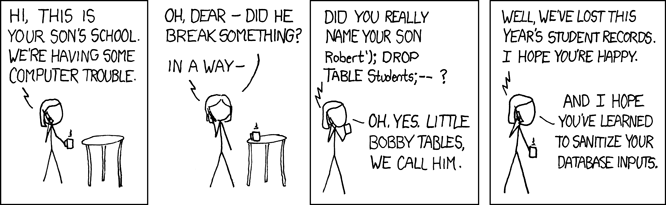
\includegraphics[width=0.6\textwidth]{bobbyTables.png}
\end{center}

Точка с запятой в SQL разделяет операторы, с ``\verb|--|'' начинается комментарий (чтобы продолжение команды не вызвало синтаксическую ошибку и DROP TABLE таки отработала). Типичный пример SQL-инъекции.

Модификация таблицы:

\begin{minted}{sql}
ALTER TABLE Students ADD email VARCHAR(MAX);
ALTER TABLE Students DROP COLUMN email;
ALTER TABLE Students ADD PRIMARY KEY (Code);
\end{minted}

Тут мы добавили новый столбец, удалили столбец, добавили ограничение, что Code является первичным ключём (следовательно, должен быть уникальным).

\section{Демонстрация}

Теперь предлагается попробовать поработать с живой СУБД, пока на уровне SQL. Это, кстати, хороший способ проверить адекватность схемы БД и правильность SQL-запросов перед тем, как пытаться реализовать что-то в коде. Для этого нам понадобится, собственно, СУБД, например, MariaDB (вообще, их десятки, но MariaDB бесплатна и довольно проста в обращении).

\begin{enumerate}
    \item Устанавливаем MariaDB (\url{https://downloads.mariadb.org/})
    \begin{enumerate}
        \item При установке спросят пароль для пользователя root, придумываем, вводим и запоминаем его
    \end{enumerate}
    \item Запускаем HeidiSQL, которая поставляется с MariaDB из коробки
    \item ``Создать'' -> ``Сеанс в корневой папке''
    \item Вводим пароль для рута, который мы запомнили на этапе 1.a.
    \item Порт 3306, по умолчанию.
    \item Видим список баз, давайте создадим новую
\end{enumerate}

Создаём тестовую БД, которую будем мучить

\begin{enumerate}
    \item Правой кнопкой на Instance сервера (Unnamed), ``Создать'' -> ``База данных''
    \item Вводим имя БД, например, ``myDB'', жмём ``ОК''
    \item База появилась в списке, создадим таблицу
    \item Клик правой кнопкой по базе, ``Создать'' -> ``Таблица''
    \item Вводим имя (например, Cities)
    \item Жмём ``Добавить'' рядом со ``Столбцы'', вводим имя столбца (id) и тип данных (INT)
    \item Снимаем галку ``Разрешить NULL''
    \item Ставим ``По умолчанию'' AUTO\_INCREMENT
    \item Кликаем по нему правой кнопкой, ``Создать новый индекс'' -> ``PRIMARY''
    \item Добавляем второй столбец, name (типа VARCHAR(50))
    \item Жмём ``Сохранить''
    \item Создадим вторую таблицу, People, со столбцами id, name и city\_id
    \item Не забываем пометить id как AUTO\_INCREMENT и PRIMARY
    \item Идём во вкладку ``Внешние ключи'', жмём ``Добавить'', пишем имя ключа ``city\_id'', ``Столбцы'' --- ``city\_id'', ``Справочная таблица'' --- ``cities'', ``Внешние столбцы'' --- ``id''
    \item Добавим немного данных
    \item ``cities'' -> ``Данные'', правый клик, ``Вставить строку'', игнорируем id, вводим ``St. Petersburg'' в name, кликаем куда-нибудь вне строки, строка добавилась
    \item Вставляем ещё Moscow и ещё что-нить
    \item ``people'' -> ``Данные'', вставляем так же пару человек
    \item Не забываем выбрать city\_id из списка, иначе операция добавления не пройдёт и вам напомнят
\end{enumerate}

Пробуем написать SQL-запрос

\begin{enumerate}
    \item Кликаем mydb, вкладку ``Запрос''
    \item Пишем там ``SELECT people.name FROM people, cities WHERE people.city\_id = cities.id AND cities.name = 'St. Petersburg'''
    \item Жмём ``Выполнить SQL'' на панели инструментов
    \item Видим таблицу с результатами нашего INNER JOIN-запроса снизу.
\end{enumerate}

\section{ADO.NET}

Теперь про то, как пользоваться реляционными базами данных из программ на C\#. Первый способ, самый простой и прямолинейный, хотя и не рекомендуемый к использованию в современных приложениях --- с помощью библиотеки ADO.NET (Active Data Objects). Библиотека довольно старая, но ей иногда пользуются и до сих пор.

ADO.NET позволяет исполнять SQL-запросы для разных источников данных --- для разных видов СУБД, даже для XML и таблиц Excel. Реализовано это за счёт архитектурного разделения запросов к данным и способа доступа к ним (например, протокола общения с конкретной СУБД). За доступ к данным и всякие низкоуровневые штуки, связанные с подключением и запросами, отвечает подсистема Data Provider-ов, которые иногда надо ставить отдельно, как NuGet-пакеты. Какой конкретно провайдер сейчас использовать и как подключиться к конкретной базе, система понимает с помощью Connection String --- просто строки, в которой указаны все атрибуты соединения. Connection String-и для всех СУБД разные (что логично, у каждой могут быть свои представления о том, что необходимо для подключения). При этом Connection String-и --- это не специфика ADO.NET, они используются и другими библиотеками для доступа к данным. Хорошая новость в том, что форматы строк подключения легко гуглятся.

Всё необходимое для работы с ADO.NET находится в пространстве имён System.Data и поставляется прямо с .NET Framework (или .NET Core). Команда к базе представляется классом Command, подключение к базе --- это подкласс Connection. Есть ещё DataSet, представляющий собой более-менее высокоуровневое представление данных --- загруженный в память набор данных из нескольких таблиц, к которому можно обращаться напрямую или выполнять LINQ-запросы.

Вот так это выглядит в коде:

\begin{minted}{csharp}
public static void Main()
{
    using (var connection = new MySqlConnection(
        "database=cities;server=localhost;user id=root;" + 
        "Password=my-secr3t-p4ssw0rd;SslMode=none"))
    {
        var command = new MySqlCommand("SELECT Id, Name FROM City", connection);
        connection.Open();
        var reader = command.ExecuteReader();
        while (reader.Read())
        {
            Console.WriteLine($"Id: {reader.GetInt32(0)}\tName:{reader.GetString(1)}");
        }
    }
}
\end{minted}

Тут мы создаём подключение к той же базе MariaDB, которую мы совсем недавно создали, создаём команду, в которой прямо пишем SELECT-запрос, исполняем её, получая объект DataReader, с помощью которого можно читать результаты запроса. DataReader ленивый в том смысле, что значения вычитываются из потока, данные в который пишет СУБД, постепенно.

А вот так выглядит запись в базу:

\begin{minted}{csharp}
public static async Task Main()
{
    using (var connection = new MySqlConnection(
        "database=cities;server=localhost;user id=root;" +
        "Password=my-secr3t-p4ssw0rd;SslMode=none"))
    {
        var command = new MySqlCommand(
            "INSERT INTO City (name) VALUES (@name)", connection);
        command.Parameters.AddWithValue("@name", "Peterhof");
        connection.Open();
        await command.ExecuteNonQueryAsync();
        Console.WriteLine($"Done, inserted row id = {command.LastInsertedId}");
    }
}
\end{minted}

Разница в том, что тут ничего читать не надо, поэтому используется метод ExecuteNonQueryAsync.

И теперь понятно, почему ADO.NET не рекомендуется использовать в современном коде --- операторы SQL надо писать прямо в программе, как строки, следовательно, их не проверяет компилятор, следовательно, очень легко ошибиться. Ну и неудобно, по сравнению со следующим способом общения с базой, ORM-системами.

\section{Entity Framework Core}

ORM (Object-Realtional Mapping) системы --- библиотеки, служащие для преобразования данных из реляционной модели в объектно-ориентированную. Они позволяют программисту работать с данными в привычном для объектно-ориентированных программ виде --- как с классами, с наследованием, отношениями ``многие-ко-многим'' и т.д. ORM-библиотека сама берёт на себя задачи по формированию SQL-кода, который читает данные из базы и пишет их туда. Это исключает возможность ошибки на уровне SQL-кода --- всё, что делает программист, он делает на своём языке программирования, и это проверяется системой типов. Недостатком такого подхода является то, что мы доверяем написание SQL-кода библиотеке, которая может делать это не оптимально. И правда, рукописный SQL, если уметь его писать, часто оказывается эффективнее, но, в конце концов, код на ассемблере, если уметь его писать, эффективнее порождённого компилятором. Так что сейчас всё-таки чаще пользуются ORM-библиотеками.

Entity Framework --- пожалуй, самая популярная ORM-библиотека под .NET, хотя и далеко не единственная (NHibernate и iBATIS, например, тоже весьма популярны). Нынче наиболее актуальная её версия --- Entity Framework Core, более старая, но более активно используемая в индустрии --- Entity Framework 6. EF Core, как следует из названия, работает на .NET Core, EF 6 --- только на полноценной .NET Framework. EF Core --- это переписанный практически с нуля EF 6, поэтому часть возможностей EF 6 там не реализована (пока что), например, отношение ``многие-ко-многим''.

Как оно работает: вы пишете у себя в коде классы, которые будут представлять данные из БД. Это внешне обычные и ничем не примечательные классы, особенно если вы следуете соглашениям касательно имён по умолчанию, которых ожидает EF Core. Далее, пишете наследника класса DbContext --- это что-то вроде точки входа в функциональность хранения данных. В нём прописывается, как подключиться к базе, в нём же указывается, к каким таблицам из базы мы хотим получить доступ. DbContext же представляет абстракцию соединения с базой, так что перед исполнением каждого запроса DbContext надо создать, а после исполнения его корректно завершить, вызвав ему Dispose (лучше, использовав using). По DbContext и класам-данным EF Core строит своё представление о БД, этот процесс называется моделированием БД. Обратите внимание, что EF Core не смотрит на саму базу, так что если код и схема БД расходятся, будет печаль. На основании этого представления EF Core будет выполнять запросы уже к реальной базе.

Вот как это выглядит на картинке из книжки J. Smith, ``Entity Framework Core In Action'':

\begin{center}
    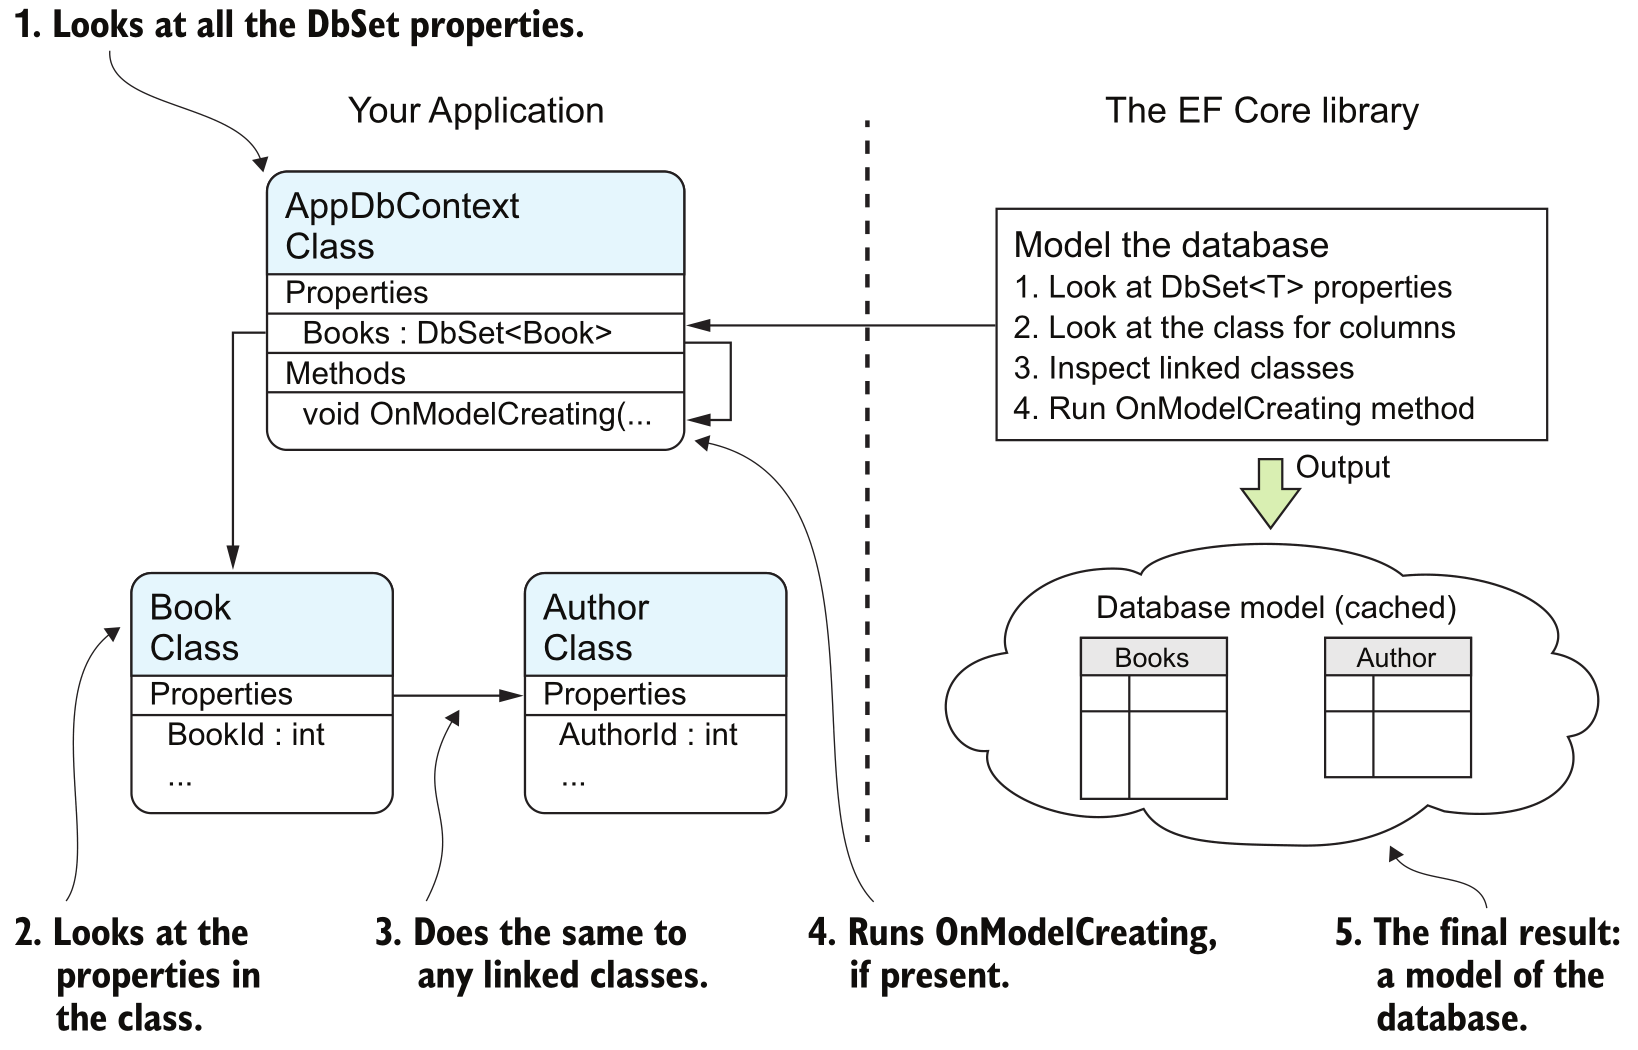
\includegraphics[width=0.8\textwidth]{efCoreDatabaseModeling.png}
\end{center}

EF Core рефлексией обходит поля классов начиная с DbContext, и интерпретирует все ссылки на другие классы как связи с другими таблицами в БД (так что таблицы, которые мы не хотим запрашивать непосредственно, явно выписывать в DbContext не надо, EF Core сама их найдёт). Свойства же элементарных типов становятся колонками в соответствующих таблицах.

А вот так на основании модели выполняется запрос (опять же, и далее в этом разделе, из ``Entity Framework Core In Action''):

\begin{center}
    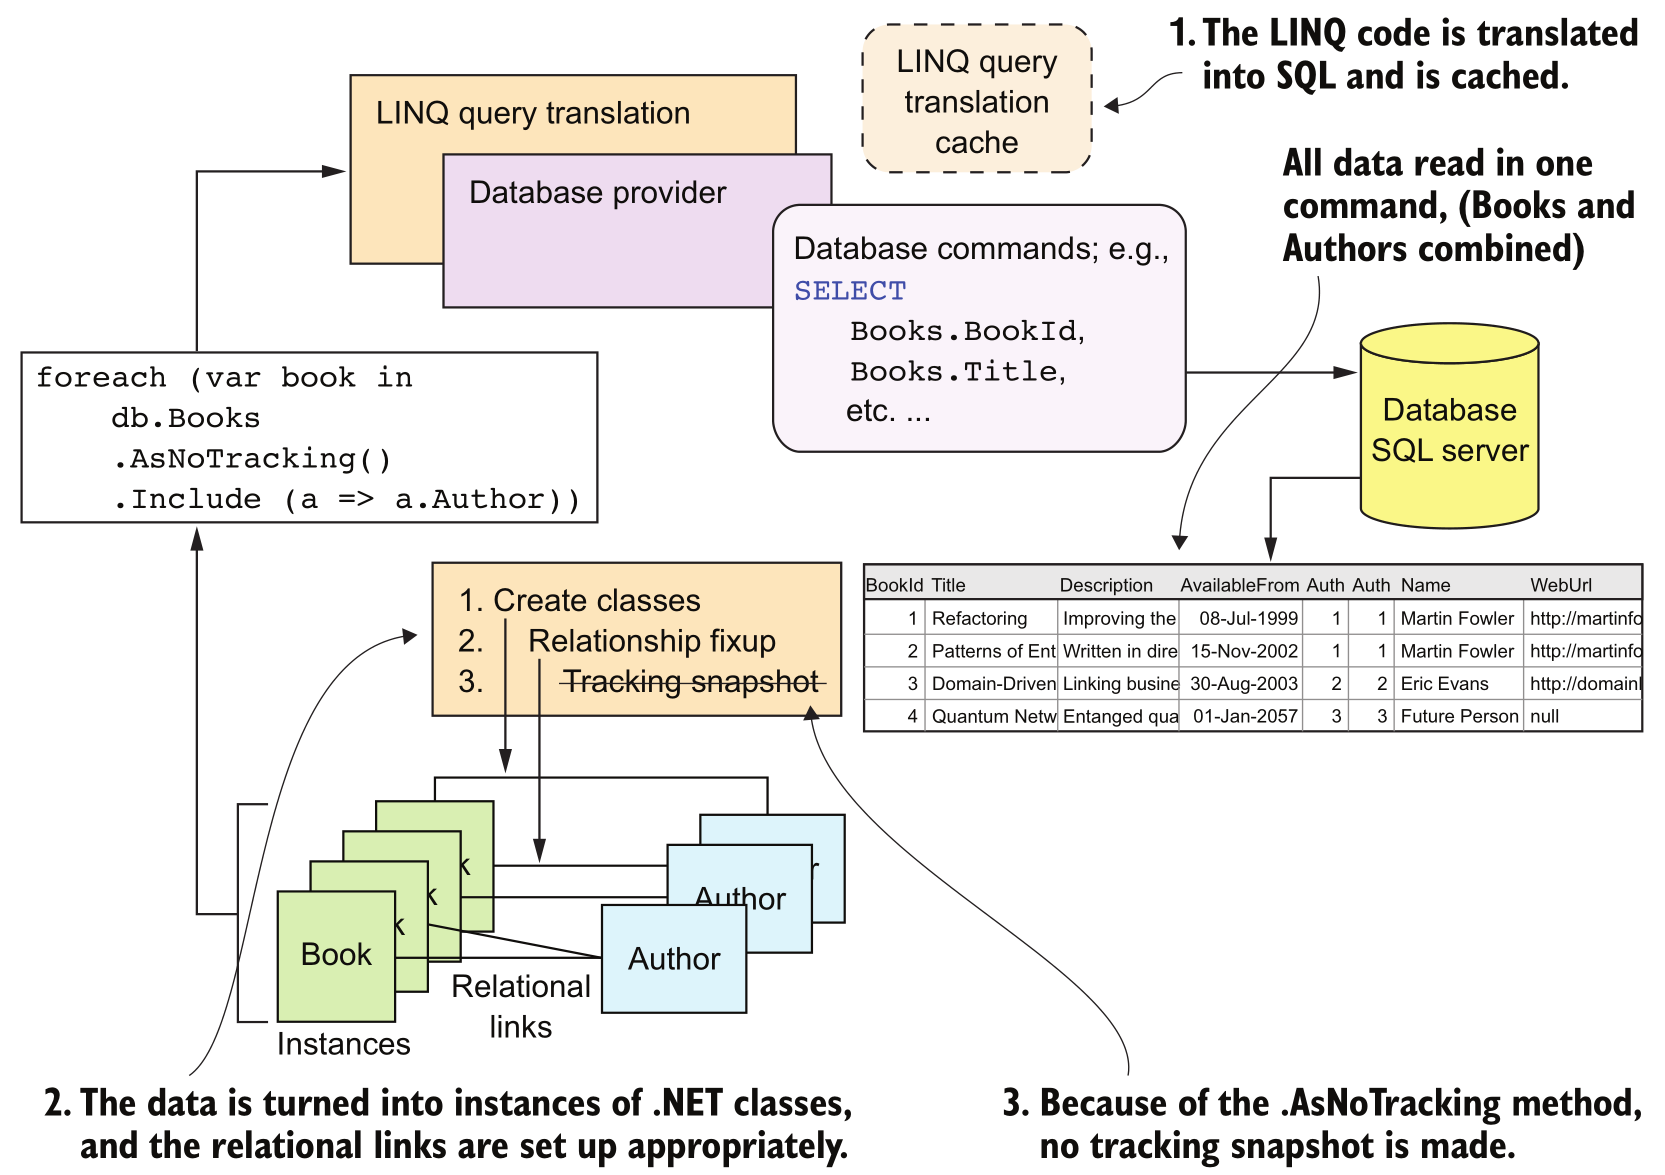
\includegraphics[width=0.8\textwidth]{efCoreQuery.png}
\end{center}

Сам запрос (точнее, программа, вычитывающая информацию из базы) мог бы выглядеть следующим образом:

\begin{minted}{csharp}
public static void ListAll()
{
    using (var db = new AppDbContext())
    {
        foreach (var book in db.Books.AsNoTracking().Include(a => a.Author))
        {
            var webUrl = book.Author.WebUrl == null 
                ? "- no web URL given -" 
                : book.Author.WebUrl;
            Console.WriteLine($"{book.Title} by {book.Author.Name}");
            Console.WriteLine("Published on " 
                + $"{book.PublishedOn:dd-MMM-yyyy}" 
                + $". {webUrl}");
        }
    }
}
\end{minted}

Запрос пишется как выражение на LINQ относительно одного из свойств DbContext-а, имеющего тип DbSet (и представляющего таблицу в базе). AsNoTracking означает, что мы не собираемся модифицировать базу, поэтому она не должна запоминать никакой информации, которая помогла бы потом применить изменения. Include(a => a.Author) означает, что EF Core должна загрузить информацию об авторах сразу же. По этому LINQ-запросу генерируется SQL-код, котоырй и делает запрос к базе, тут он получается вот такой:

\begin{minted}{sql}
SELECT b.BookId,
    b.AuthorId,
    b.Description,
    b.PublishedOn,
    b.Title,
    a.AuthorId,
    a.Name,
    a.WebUrl
FROM Books AS b
INNER JOIN Author AS a ON
    b.AuthorId = a.AuthorId
\end{minted}

Запрос выполняется, результаты его складываются в объекты Book и Author, между ними устанавливаются правильные связи (магией рефлексии), затем результат возвращается как результат запроса.

Теперь более интересный случай, обновление БД. Положим, мы хотим поменять URL у наших книг в базе (да, я схему БД для этих примеров не привёл, но она довольно очевидна, слегка видна на картинках и к тому же, это хороший повод почитать книжку). Код на C\# будет выглядеть так:

\begin{minted}{csharp}
public static void ChangeWebUrl()
{
    Console.Write("New Quantum Networking WebUrl > ");
    var newWebUrl = Console.ReadLine();
    using (var db = new AppDbContext())
    {
        var book = db.Books.Include(a => a.Author)
                           .Single(b => b.Title == "Quantum Networking");
        book.Author.WebUrl = newWebUrl;
        db.SaveChanges();
        Console.WriteLine("... SavedChanges called.");
    }
}
\end{minted}

Тут мы уже не делаем AsNoTracking() (поскольку собираемся менять базу), зато добавляем к запросу \mintinline{csharp}|Single(b => b.Title == "Quantum Networking");|, чтобы найти ту самую книгу, которую мы собираемся модифицировать (если их оказалось несколько или ни одной, будет брошено исключение). Меняем ей URL (обратите внимание, это просто запись в свойство, и это правда самое обычное свойство), а дальше вызываем SaveChanges у DbContext-а, который и отправляет изменения в БД. При этом, пока мы не вызывали SaveChanges, изменения существуют только в памяти. SaveChanges может сохранять сразу пачку изменений и чаще всего обладает свойством транзакционности: либо все изменения принимаются БД, либо ни одно, и тогда БД не изменяется.

Вот как это выглядит на картинке:

\begin{center}
    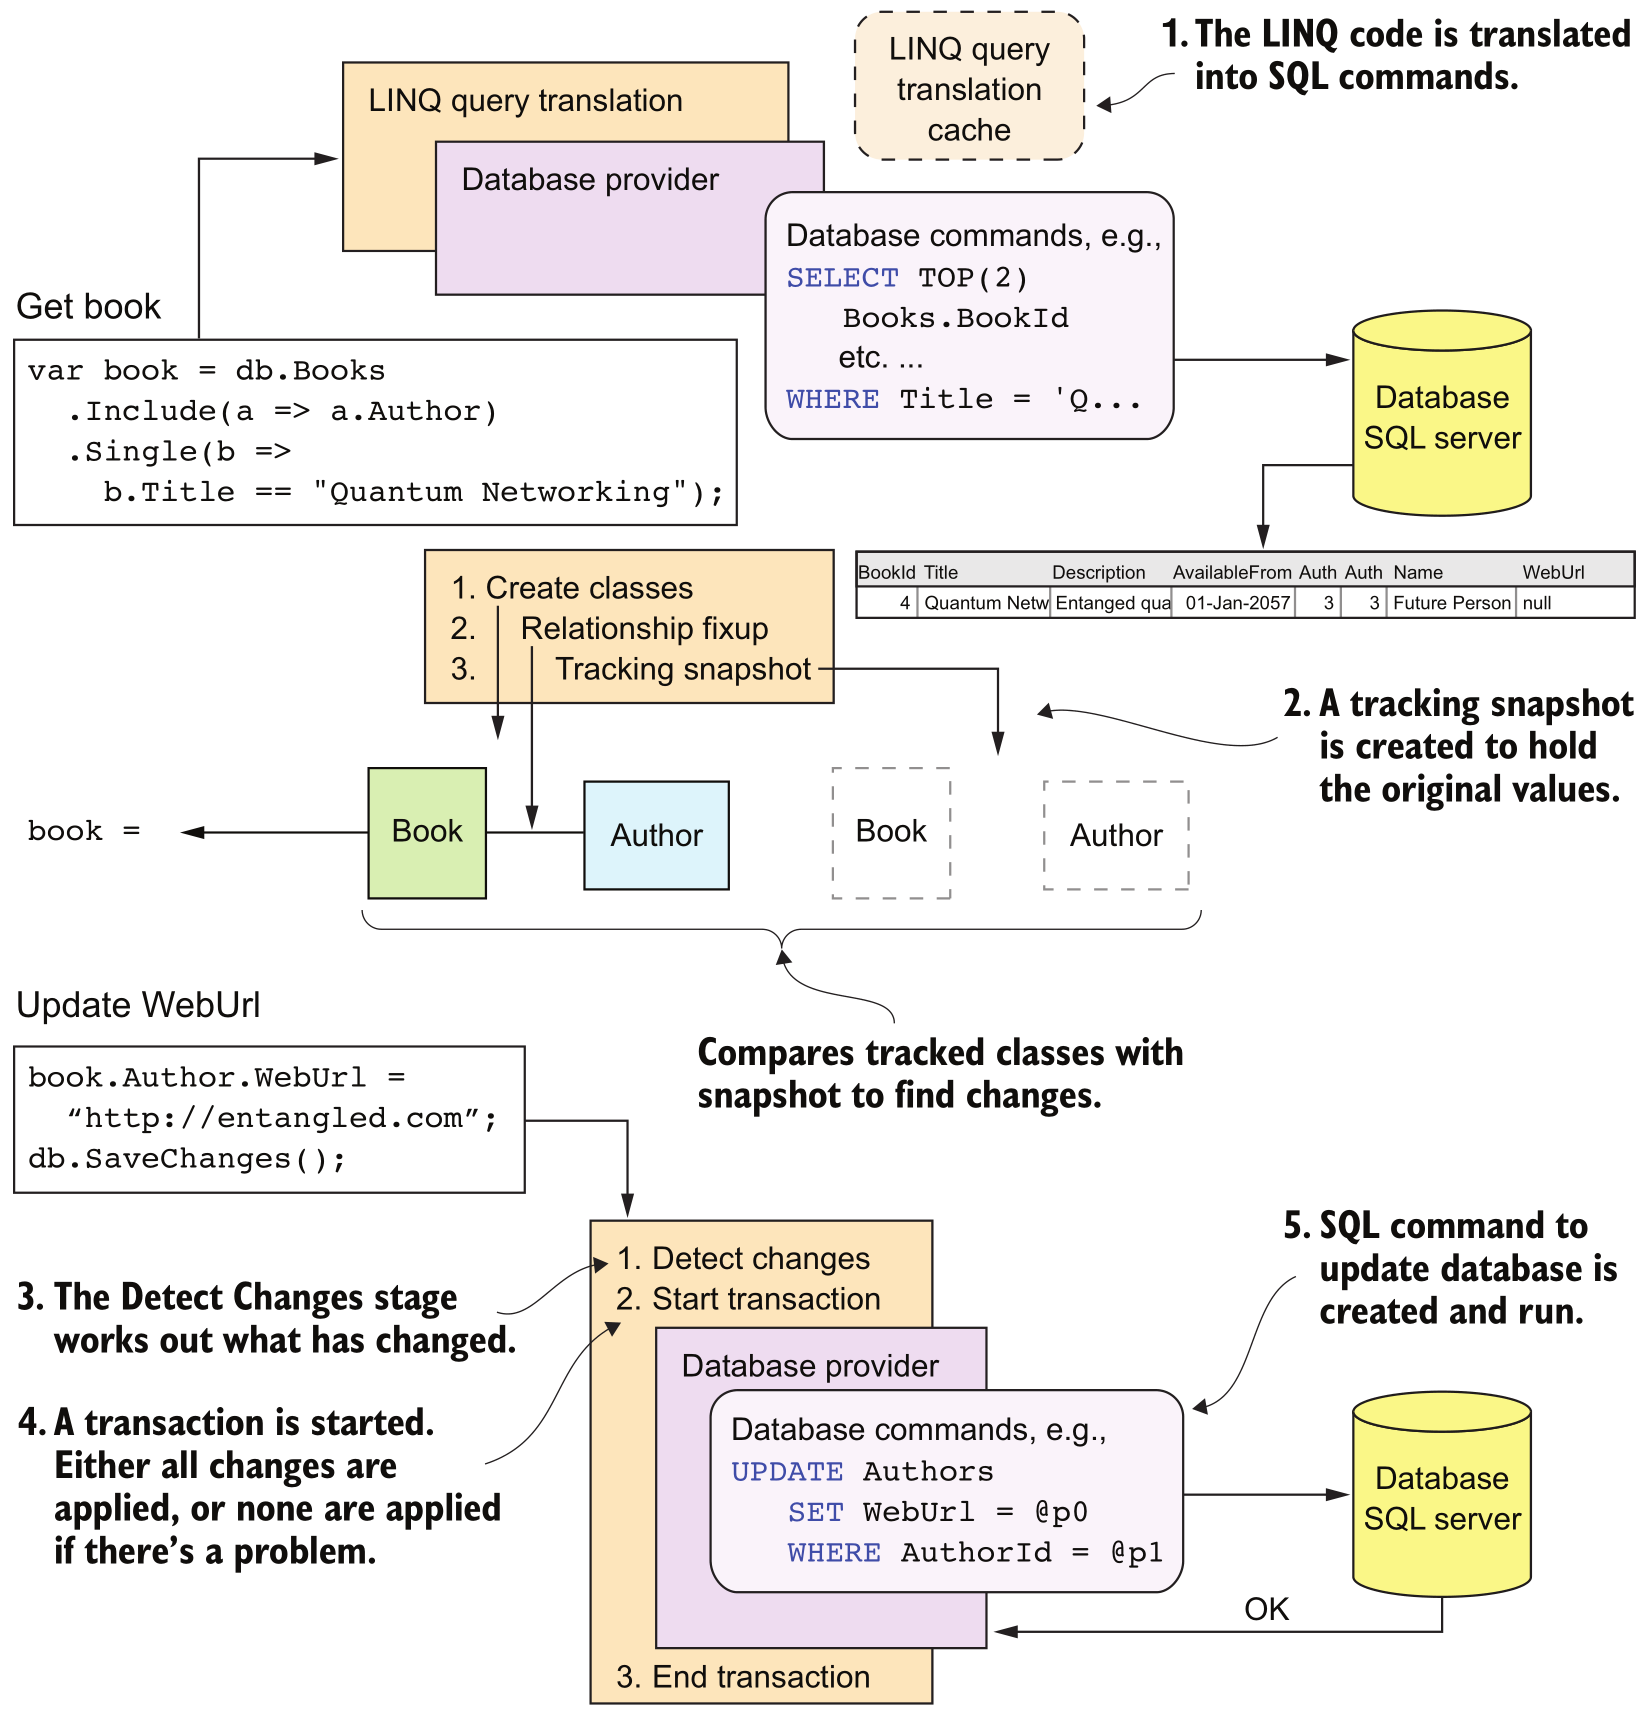
\includegraphics[width=0.8\textwidth]{efCoreUpdate.png}
\end{center}

Каак видим, EF Core работает примерно как git, считая автоматически изменения между данными в базе и в памяти, и записывая в базу только изменения.

\subsection{Демонстрация}

А теперь давайте попробуем сделать приложение, работающее с EF Core, с нуля.

Создадим проект как консольное приложение .NET Core. Пойдём в Manage NuGet Packages и поставим провайдер для той базы, с которой мы хотим работать. Начнём с уже известной нам MariaDB, так что ставим Pomelo.EntityFrameworkCore.MySql (помним, что MariaDB --- это форк MySQL, поэтому всё, что работает для MySQL, скорее всего, будет работать и для неё). При этом зависимостями скачается и сама EF Core, и всё, что ей нужно для работы.

Описываем наши классы, которые будут представлять таблицы из БД:

\begin{minted}{csharp}
public class City
{
    [Column("id")]
    public int CityId { get; set; }

    public string Name { get; set; }
}

public class Person
{
    public int PersonId { get; set; }

    [Column("person_name")]
    public string PersonName { get; set; }

    [Column("city_id")]
    public int CityId { get; set; }

    public City City { get; set; }
}
\end{minted}

По соглашениям EF Core свойства вида <имя класса>Id станут в базе суррогатными первичными ключами, <имя другого класса>Id станут внешними ключами, а свойство \mintinline{csharp}|public City City { get; set; }| называется навигационным свойством --- свойством, которое позволяет ходить по связям между таблицами. Ещё с помощью атрибута Column нам пришлось переименовать несколько полей, потому что в базе они называются ужасно.

Дальше DbContext:

\begin{minted}{csharp}
class PersonCityDbContext: DbContext
{
    public DbSet<Person> Person { get; set; }

    protected override void OnConfiguring(DbContextOptionsBuilder optionsBuilder)
    {
        optionsBuilder.UseMySql("database=cities;server=localhost;user id=root;" +
                "Password=my-secr3t-p4ssw0rd;SslMode=none");
    }
}
\end{minted}

Свойство типа DbSet<Person> должно называться так же, как таблица в базе, это позволяет EF Core легко найти, к чему мы там обращаемся. optionsBuilder.UseMySql хочет Connection String, и она внезапно оказывается той самой строкой, которую мы использовали для ADO.NET. Это не удивительно, ведь EF Core использует Data Provider-ы из ADO.NET, чтобы общаться с базой.

А теперь сам код чтения из базы:

\begin{minted}{csharp}
using (var context = new PersonCityDbContext())
{
    foreach (var person in context.Person.AsNoTracking().Include(a => a.City))
    {
        Console.WriteLine($"{person.PersonName} lives in {person.City.Name}");
    }
}
\end{minted}

Тут вроде как ничего неожиданного. Давайте ещё добавим запись для полноты картины:

\begin{minted}{csharp}
using (var context = new PersonCityDbContext())
{
    var newPerson = new Person() { PersonName = "Alexey" };
    var city = await context.Person
        .Include(p => p.City)
        .SingleAsync(p => p.PersonName == "Andrey")
        .ContinueWith(p => p.Result.City);
    Console.WriteLine($"Adding {newPerson.PersonName} living in {city.Name}");
    newPerson.City = city;
    context.Person.Add(newPerson);
    await context.SaveChangesAsync();
}
\end{minted}

Тут мы создаём нового человека и заставляем его жить там же, где живёт некий Андрей (в надежде, что в базе всего один Андрей). Находим город Андрея и добавляем ссылку на него как город Алексея, сохраняем изменения в базу. Проверяем в HeidiSql, Алексей появился. Если написать .AsNoTracking() при поиске города, всё упадёт, потому что EF Core попытается добавить такой город ещё раз (раз он не трекает объект, он думает, что это новый и его надо добавить в базу).

А теперь давайте сделаем это же с помощью Sqlite --- базы данных, которую вообще не надо отдельно ставить и конфигурировать, заводить там пользователей и т.д. и т.п., которая просто качается как NuGet-пакет и  может быть использована в любом .NET-приложении (сама СУБД будет просто лежать с ним рядом как обычная .dll-ка).

Сначала добавим провайдер Microsoft.EntityFrameworkCore.Sqlite, который заодно и поставит саму Sqlite.

Дальше поменяем Connection String в DbContext:

\begin{minted}{csharp}
class PersonCityDbContext: DbContext
{
    public DbSet<Person> Person { get; set; }

    protected override void OnConfiguring(DbContextOptionsBuilder optionsBuilder)
    {
        optionsBuilder.UseSqlite("Data Source=cities.db");
    }
}
\end{minted}

Дальше, не меняя модель данных, попробуем что-нить добавить и что-нить прочитать:

\begin{minted}{csharp}
public static async Task Main(string[] args)
{
    using (var context = new PersonCityDbContext())
    {
        context.Database.EnsureCreated();
        var newPerson = new Person() { PersonName = "Alexey" };
        var newCity = new City() { Name = "St. Petersburg" };
        newPerson.City = newCity;
        context.Person.Add(newPerson);
        await context.SaveChangesAsync();
    }

    using (var context = new PersonCityDbContext())
    {
        foreach (var person in context.Person.AsNoTracking().Include(a => a.City))
        {
            Console.WriteLine($"{person.PersonName} lives in {person.City.Name}");
        }
    }
}
\end{minted}

Видно, что по сути ничего не изменилось, но теперь пользоваться нашим приложением будет существенно проще, потому что не надо ставить отдельную СУБД.

\end{document}
